\begin{vidu}
\immini[thm]{
Gờ giảm tốc như hình bên có tác dụng cảnh báo (thông qua việc gây ra tác động nhẹ lên phương tiện) cho người tham gia giao thông biết trước đoạn đường này nguy hiểm, cần phải giảm tốc độ và chú ý quan sát để bảo đảm an toàn giao thông.
Một ô tô có khối lượng 1465 kg chở hai người có tổng khối lượng 110 kg đi qua một đoạn đường có gờ giảm tốc, với những nếp gấp cách nhau 0,50 m. Ô tô này nảy lên với biên độ cực đại khi tốc độ của nó là 20 km/h.}{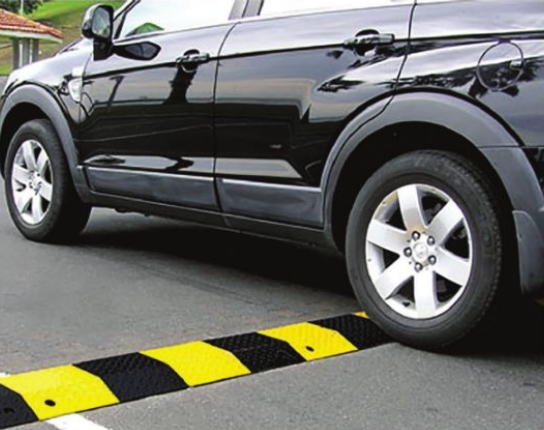
\includegraphics[width=4cm]{Hinh/CDH4}}  

Ta có thể coi gần đúng hệ thống này như một con lắc lò xo có chu kì dao động tính bằng công thức: $T=2\pi\sqrt{\dfrac{m}{k}}$. Xác định độ cứng tương đương của hệ thống lò xo gắn với khung xe. 

\loigiai{
Hiện tượng cộng hưởng: $T=T_0\Rightarrow 2\pi\sqrt{\dfrac{m}{k}}=\dfrac{s}{v}\Rightarrow k=\dfrac{4\pi^2.m.v^2}{s^2}=\dfrac{4\pi^2.(110+1465).\left(\dfrac{50}{9}\right)^2}{0,5^2}=7676359\ N/m$.
}
%\haidong{4}
\end{vidu} %\dotlineEX{3}
%\loai{Dao động cưỡng bức - cộng hưởng}
\begin{vidu}%[3P1-21.2B][Loai1]
Một con lắc lò xo gồm vật nhỏ có khối lượng m, lò xo có khối lượng không đáng kể, độ cứng $k = 10\ N/m$. Con lắc dao động cưỡng bức dưới tác dụng của ngoại lực tuần hoàn có tần số góc $ \omega _f$. Biết biên độ của ngoại lực tuần hoàn không thay đổi. Khi thay đổi tần số góc $ \omega _f$ thì biên độ dao động của vật nhỏ thay đổi và khi $ \omega _f=10\ rad/s$ thì biên độ dao động của vật nhỏ đạt cực đại. Khối lượng m của vật nhỏ là
\choice
{120 g}
{40 g}
{10 g}
{\True 100 g}
\loigiai{
\begin{itemize}
\item Biên độ dao động của vật đạt cực đại khi hiện tượng cộng hưởng xảy ra. 
\item Khi đó: $ \omega _f= \omega _0=\sqrt{\dfrac{k}{m}}\Rightarrow m=\dfrac{k}{\omega _f^2}=\dfrac{10}{10^2}=0,1\ kg=100\ g$.
\end{itemize}
}
%\haidong{4}
\end{vidu} %\dotlineEX{3}
\begin{vidu}%[3P1-21.2B][Loai1]
Một con lắc dài 44 cm được treo vào trần của một toa xe lửa. Con lắc bị kích động mỗi khi bánh của toa xe gặp chỗ nối nhau của đường ray. Hỏi tàu chạy thẳng đều với tốc độ bằng bao nhiêu thì biên độ dao động của con lắc sẽ lớn nhất. Cho biết chiều dài của mỗi đường ray là 12,5 m. Lấy $g = 9,8$ $m/s^2$.
\choice
{10,7 km/h}
{\True 34 km/h}
{106 km/h}
{45 km/h}
\loigiai{
Biên độ dao động của con lắc sẽ lớn nhất khi xảy ra cộng hưởng:
\begin{align*}
T={T_0}\Leftrightarrow \dfrac{S}{v}=\dfrac{2\pi}{\omega}=\dfrac{2\pi}{\sqrt{\dfrac{g}{\ell}}}\Rightarrow v=\dfrac{s\sqrt{\dfrac{g}{\ell}}}{2\pi}=9,4\ m/s =33,84\ km/h \approx 34\ km/h.
\end{align*}
}
%\haidong{4}
\end{vidu} %\dotlineEX{5}
%\loai{So sánh biên độ}
\begin{vidu}%[3P1-19.2K][Loai1]
Một con lắc đơn có chiều dài $\ell =16$ cm dao động trong không khí. Cho $g\approx 10\ m/s^2;\ \pi^2\approx 10.$ Tác dụng lên con lắc một ngoại lực biến thiên tuần hoàn có biên độ không đổi nhưng tần số $f$ có thể thay đổi. Khi tần số của ngoại lực lần lượt có giá trị $f_1=0,7\ Hz$ và $f_2 = 1$ Hz thì biên độ dao động của vật tương ứng là $A_1$ và $A_2$. So sánh $A_1$ và $A_2$?
\choice
{$A_1\ge A_2$}
{\True $A_1<A_2$}
{$A_1=A_2$}
{$A_1>A_2$}
\loigiai{
\begin{itemize}
\item Tần số dao động riêng của vật: $f_0=\dfrac{\omega}{2\pi}=\dfrac{\sqrt{\dfrac{g}{\ell}}}{2\pi}=1,25\ Hz $.
\item Biên độ dao động của hệ phụ thuộc vào độ chênh lệch giữa tần số dao động riêng của vật $f_0$ và tần số f dao động của ngoại lực (hay $|f - f_0|$).
\item Khi tần số của lực cưỡng bức càng gần tần số dao động riêng thì biên độ dao động cưỡng bức càng lớn. 
\item Ta có $ \left| f_1-f_0 \right|>\left| f_2-f_0 \right|\Rightarrow A_1<A_2$.
\end{itemize}
}
%\haidong{6}
\end{vidu} %\dotlineEX{5}
%\loai{\% cơ năng bị giảm}
\begin{vidu}%[3P1-21.2K][Loai1]
Một con lắc dao động tắt dần. Cứ sau mỗi chu kì, biên độ giảm 3\%. Phần năng lượng của con lắc bị mất đi trong một dao động toàn phần là
\choice
{3\%}
{9\%}
{4,5 \%}
{\True 6\%}
\loigiai{
\begin{itemize}
\item Ta có: $A' = 97\% A \Rightarrow E' = \dfrac{1}{2}kA'^2 = \dfrac{1}{2}k\left(97\% A \right)^2 = 94,09\%\dfrac{1}{2}kA^2\Rightarrow \dfrac{\Delta E}{E} = 5,91\% \approx 6\%$.

\end{itemize}
}
%\haidong{4}
\end{vidu} %\dotlineEX{5}
\begin{vidu}%[3P1-20.1K][Loai1]
Một con lắc dao động tắt dần. Cứ sau mỗi chu kì biên độ giảm 2\% so với lượng còn lại. Sau 5 chu kì, so với năng lượng ban đầu, năng lượng còn lại bằng
\choice
{78,6\%}
{69,2\%}
{74,4\%}
{\True 81,7\%}
\loigiai{
\begin{itemize}
\item Sau mỗi chu kì biên độ giảm 2\% so với lượng còn lại. như vậy sau 5 chu kì thì biên độ của vật lúc này là $A_5 = 0,98^5.A = 0,9039A.$ 
\item Năng lượng lúc này là $W_5 = \dfrac{KA^2_5}{2} = 0,817.\dfrac{KA^2}{2}$
$\Rightarrow$Năng lượng còn lại là 81,7\%.
\end{itemize}
}
%\haidong{6}
\end{vidu} %\dotlineEX{8}
%\loai{Quãng đường vật đi được cho đến khi dừng lại}
\begin{vidu}%[3P1-20.1K][Loai1]
Một con lắc lò xo dao động trên mặt sàn nằm ngang gồm một lò xo nhẹ có độ cứng $k=10\ N/m$, một đầu gắn cố định, đầu còn lại gắn một vật khối lượng $m=100\ g$. Hệ số ma sát giữa vật với mặt sàn là $\mu =0,1$. Ban đầu đưa vật đến vị trí lò xo bị nén một đoạn 7 cm và thả ra. Lấy $g=10\ m/s^2$. Quãng đường vật đi được cho đến khi vật dừng lại là
\choice
{32,5 cm}
{\True 24,5 cm}
{24 cm}
{32 cm}
\loigiai{
\begin{itemize}
\item Quãng đường vật đi được đến khi dừng hẳn: $s=\dfrac{kA^2}{2\mu mg}$.
\item Thay số vào ta được: $s=\dfrac{kA^2}{2\mu mg}=\dfrac{10.0,07^2}{2.0,1.0,1.10}=0,245\ m=24,5\ cm$.

\end{itemize}
}
%\haidong{6}
\end{vidu} %\dotlineEX{6}
